\documentclass[border=6pt]{standalone}
\usepackage{amsmath,amssymb}
\usepackage{tikz}
\begin{document}
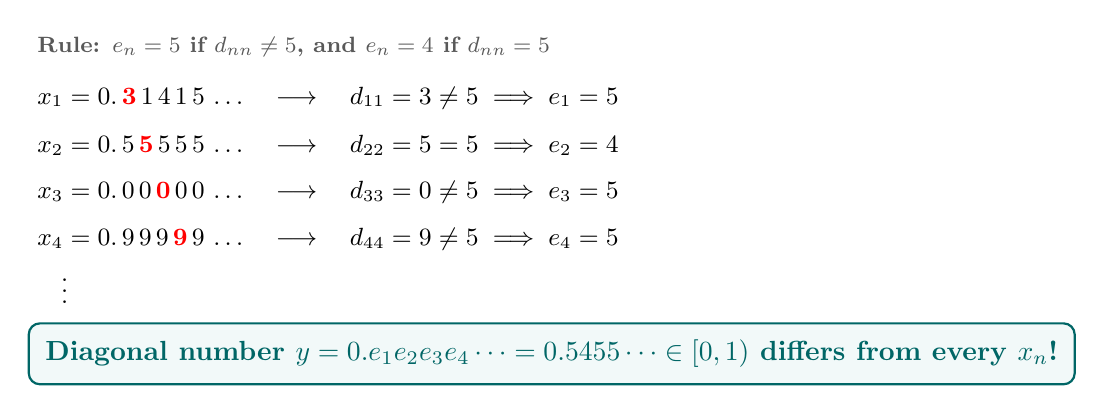
\begin{tikzpicture}[font=\small]
  \node[anchor=west, font=\footnotesize\bfseries, text=gray!70!black] at (0, 3.65)
    {Rule: $e_n = 5$ if $d_{nn} \ne 5$, and $e_n = 4$ if $d_{nn} = 5$};

  \node[anchor=west] at (0, 3.0) {$x_1 = 0.\,\mathbf{\color{red}3}\,1\,4\,1\,5\,\dots \quad \longrightarrow \quad d_{11} = 3 \ne 5 \implies e_1 = 5$};
  \node[anchor=west] at (0, 2.4) {$x_2 = 0.\,5\,\mathbf{\color{red}5}\,5\,5\,5\,\dots \quad \longrightarrow \quad d_{22} = 5 = 5 \implies e_2 = 4$};
  \node[anchor=west] at (0, 1.8) {$x_3 = 0.\,0\,0\,\mathbf{\color{red}0}\,0\,0\,\dots \quad \longrightarrow \quad d_{33} = 0 \ne 5 \implies e_3 = 5$};
  \node[anchor=west] at (0, 1.2) {$x_4 = 0.\,9\,9\,9\,\mathbf{\color{red}9}\,9\,\dots \quad \longrightarrow \quad d_{44} = 9 \ne 5 \implies e_4 = 5$};
  \node[anchor=west] at (0.3, 0.65) {$\vdots$};

  \node[anchor=west, draw=teal!80!black, thick, rounded corners=4pt, fill=teal!5, inner sep=6pt, font=\bfseries, text=teal!80!black] at (0, -0.25)
    {Diagonal number $y = 0.e_1 e_2 e_3 e_4 \dots = 0.5455\dots \in [0,1)$ differs from every $x_n$!};
\end{tikzpicture}
\end{document}
